
\section{Introduction}
Let us consider a linear recognition algorithm by Corneil, Perl, and Stewart \cite{corneil_perl_stewart_85}. Historically, this was the first linear algorithm for cograph recognition that was ever designed. Its main ideas are intuitive, but it is very difficult to implement due to the large number of cases. The proof of this algorithm is difficult for the same reason: there are many cases with many subcases.
\section{Idea}

The algorithm idea is that any induced subgraph of a cograph is a cograph, which follows, for example, from the definition about $P_4$-free graph. So we will process the vertices one by one and modify the cotree, and if it ceases to be a cograph, the algorithm stops. Our algorithm will check this condition after every inserting of vertex from $V$.

The algorithm consists of several parts: \texttt{MARK}, \texttt{FIND-LOWEST}, \texttt{ADD-VERTEX}. Let us look at each of the parts in turn.

\section{Function \texttt{MARK}}
\subsection{Idea}
Consider an algorithm iteration for vertex $x$. Assume we have a cotree $T$ for some induced subgraph of our graph $G$. We want to give the vertices of $T$ some states, which are: ``not-marked'', ``marked'' and ``marked-and-unmarked''. At the beginning all vertices are ``not-marked'' and then immediately we change the state of every neighbour of $x$ to ``marked''. 

There are two other cases when we change vertex state, and if vertex satisfies the given condition, then the changing must be applied. We change vertex state from ``not-marked'' to ``marked'' when at least one child of this vertex has state ``marked-and-unmarked''. We change vertex state from ``marked'' to ``marked-and-unmarked'' when all children of this vertex have state ``marked-and-unmarked''. 


Let us denote \emph{subtree leaves} by $L(x)=\{y : y$ is a leaf and is in the subtree rooted in $x\}$. 
So, we can create a table explaining what the vertex state means after \texttt{MARK} ends. 

\begin{center}
    \begin{tabular}{ | p{45mm} | p{60mm} | }
    \hline
    Vertex $y$ state & How many neighbours of $x$ are in $L(y)$:  \\ [0.5ex] 
    \hline\hline
    ``not-marked'' & zero \\
    \hline
    ``marked'' & at least one \\
    \hline
    ``marked-and-unmarked'' & $|L(y)|$, i.e. all \\
    \hline
    \end{tabular}
\end{center}
\subsection{Implementation}

We denote by $d(w)$ the number of children of $w$ in the cotree and by $md(w)$ the number of ``marked-and-unmarked'' children of $w$ if $w$ is ``marked'' -- otherwise we assume it is equal to $0$. 

When we consider a new vertex $x$, then we need to change the state of every $y$ from $N(x)$, that already exists in cotree, to ``marked''. Further, while there exists a ``marked`` node $v$ for which $d(v) = md(v)$, we change the state of $v$ to ``marked-and-unmarked'' and if its parent $p$ state is ``unmarked'', then we change its state to ``marked''. Otherwise, we just increase $md(p)$ by one. Note that when we change the state of $v$ to ``marked-and-unmarked'', then its parent $p$ now can have $d(p) = md(p)$, so we cannot just remember once all ``marked'' nodes $v$ with $d(v) = md(v)$, but we need to constantly update our list of such vertices.

The root has only one child if and only if the graph is disconnected. If after the end of the algorithm there is a marked node and the graph is disconnected, then we change the root of the tree state to ``marked''.

\subsection{Pseudocode}
\begin{minted}[
frame=lines,
framesep=2mm,
baselinestretch=1.2,
fontsize=\footnotesize,
linenos
]{c++}
M(v) = linked list of children of v;
MARK(x) {
  Mark all leaves of T which are adjacent to x;
  For (each marked node u of T with d(u) == md(u)) {
    unmark(u);  // change state from marked to marked-and-unmarked
    md(u) = 0;
    if (u != root) {
      mark (parent (u));
      md(w) += 1;
      insert u at the head of M(w);
    }
  }
  If (any vertex is marked and d(root) == 1) {
    mark(root); // change state from unmarked to marked-and-unmarked
  }
}
\end{minted}


\section{Function \texttt{FIND-LOWEST}}

\subsection{Idea}
The next part of our algorithm is a function \texttt{FIND-LOWEST}. Its idea is that by relying on states of vertices in cotree $T$ after calling \texttt{MARK}($x$), we check whether the graph ceases to be a cograph when adding our vertex. The theorems in \Cref{Correnctness} help us to determine whether after adding $x$ to $G$ it ceases to be cograph. We either return that $G+x$ is not a cograph or we return a node $\alpha$ -- the lowest marked node of cotree. 



\subsection{Implementation}
Let us introduce the following definitions and notation.
\begin{definition}
    A node $y$ is \emph{properly marked} if and only if it is a $(1)$-node, it is marked and $md(y) = d(y) - 1$. 
\end{definition}

\begin{definition}
    A \emph{legitimate alternating path} is a path of adjacent alternating properly marked $(1)$-nodes and not ``marked'' $(0)$-nodes, the extreme points of which are $(1)$-nodes.
\end{definition}
 Let us denote the graph by $G$, a cotree of $G$ by $T$. Let $x$ be the current vertex we are trying to insert to $G$, $u$ be the lowest marked node so far examined, $w$ be the previous value of $u$; i.e. the lowest marked node examined before $u$. Let $y$ be a marked $(1)$-node which is not properly marked or a marked $(0)$-node, if either exists in cotree.

At each step of the algorithm we choose $u$ and $w$ from $T$ and check if the path between them is a legitimate alternating path. At the first step $w$ is initialized to the root and $u$ initialized to any marked node. At another step we make $w$ equal to $u$, and $u$ equal to another arbitrary marked node. At the end of each step we change the state of $u$ to ``marked-and-unmarked''.

Let us divide the function into phases. The first phase is initialization. The second phase is choosing arbitrary marked vertex $u$ and checking some conditions for it. The third phase is checking if the path between $u$ and $w$ is a legitimate alternating path and unmarking vertices along this path. 

\subsection{Pseudocode}

\begin{minted}[
frame=lines,
framesep=2mm,
baselinestretch=1.2,
fontsize=\footnotesize,
linenos
]{c++}
FIND-LOWEST() {
  // Phase 1.
  y = trash;
  If (R is not marked) {
    // G+x is not a cograph: condition (iii)
    return NOT_COGRAPH;
  }
  if (md(R) != d(R) - 1) {
    y = R;
  }
  unmark(R);  // change state from marked to marked-and-unmarked
  md(R) = 0;
  u = w = R;
  while (marked vertex exists in T) {
  // Phase 2
  u = arbitrary marked vertex;
  if (y != trash) {
    // G+x is not a cograph: condition (i) or (ii)
    return NOT_COGRAPH;
  }
  if (label (u) == 1) {
    if (md(u) != d(u) - 1) {
      y = u;
    }
    if (parent (u) is marked) {
      // G+x is not a cograph: conditions (i) and (vi)
      return NOT_COGRAPH;
    }
    else {
      t = parent (parent (u));
    }
  }
  else {
    y = u;
    t = parent (u);
  }
  unmark (u);
  md (u) = 0;
  // phase 3
  while (t != w) {
    if (t == R) {
      // G+x is not a cograph: condition (iv)
      return NOT_COGRAPH;
    }
    if (t is not marked) {
      // G+x is not a cograph: condition (iii) or (v) or (vi)
      return NOT_COGRAPH;
    }
    if (md(t) != d(t) - 1) {
      // G+x is not a cograph: condition (ii)
      return NOT_COGRAPH;
    }
    if (parent (t) is marked) {
      // G+x is not a cograph: condition (i)
      return NOT_COGRAPH;
    }
    unmark(t); 
    md(t) = 0;
    t = parent (parent (t));
  }
  // Reset w for next choice of marked vertex
  w = u;
  }
}
\end{minted}

\section{Function \texttt{ADD-VERTEX}}
\subsection{Implementation}
This method builds the next part of cotree $T$ from the bottom by combining everything that was said above. It adds vertices one at a time by calling at the beginning \texttt{MARK} function and then, after handling edge cases, it calls the second function \texttt{FIND-LOWEST}. Next, it adds a vertex to the cotree in such a way that the rules of the cotree are fulfilled, in particular, rule 3 about LCA. 

\subsection{Pseudocode}
\begin{minted}[
frame=lines,
framesep=2mm,
baselinestretch=1.2,
fontsize=\footnotesize,
linenos
]{c++}
ADD-VERTEX(V = (v1, .., vn), E) {  // V-vertices, E-edges 
  // initialization
  Create a new (1) cotree node R;
  if (v1 and v2 are neighbours) {
    add v1, v2 as children of R;
  }
  else{
    create a new (0) cotree node N;
    add N as a child of R; 
    add v1 and v2 as children of N;
  }
  // iteratively incorporate v3, .., vn into T
  for (x in (v3,...,vn)) {
    MARK (x);
    if (all nodes of T were marked and unmarked) {
      add x as a child of R;
      continue;
    }
    if (no nodes of T were marked) {
      if (d(R) == 1) {
        add x as a child of the only child of R;
      }
      else {
        create a new (label(u) ^ 1) node R with one child and
        two grandchildren: x and the old root;
      }
      continue;
    }
    u = FIND-LOWEST();
    A[0] = marked-and-unmarked children of u;
    A[1] = unmarked children of u;
    if (A[label(u)].size == 1) {
      if (w is a leaf and A[label(u)] == {w}) {
        add a new (1) cotree node ((0) cotree node) in place of w 
        and make w and x children of this node;
      }
      else {
        add x as a new child of w;
      }
    }
    else {
      remove all elements of A[0] from u; 
      add these removed elements as children of a new (label(u)) node y;
      if (u is a (0)-node) {
        add a new (1) cotree node as a child of u;
        add x and y as children of this new (1)-node;
      }
      else {
        remove u from its parent and add y in its place;
        add a new (0)-node as a child of y; 
        add x and u as children of this new (0)-node;
      }
    }
  }
}
\end{minted}

\label{Correnctness}
\section{Correctness}
\subsection{\texttt{MARK}}

Note that for vertex $v$ the condition $d(v) = md(v)$ means that all children of $v$ are ``marked-and-unmarked''. For every child $w$ of $v$ it means that it once had $d(w) = md(w)$, so all its children are ``marked-and-unmarked''. And applying such logic recursively to children of $w$ and so on, we get that every $y$ from $L(v)$ is ``marked-and-unmarked'', so once it was ``marked'', but a leaf in the tree was once ``marked'' if and only if it is the neighbour of $x$ and hence $y$ is a neighbour of $x$. 

Accordingly, if we look again at the two types of state changes that were declared in the section \texttt{MARK} we can see that vertex can become ``marked'' if it is a leaf and a neighbour of $x$, or if at least one of its children is ``marked-and-unmarked''. Hence, for this ``marked-and-unmarked'' child $w$ of $v$, as it was said above, we know that $L(w)$ consists only from children of $x$.

\subsection{\texttt{FIND-LOWEST} implementation}
As the first step we checked if the path between $u$ and root is correct, at the second step we made $w$ equals to $u$ and $u$ equals to any marked node. And we again checked if the path between $u$ and $w$ is correct; Thus, since the path between $u$ and $w$ is correct and the path between $w$ and $root$ is correct, then the path between $u$ and $root$ is correct, and so on. In this way we checked the condition $2.1$ from the \Cref{theorem_adding}.

\subsection{Theorem for \texttt{FIND-LOWEST}}
        
In order to state the theorem, we need to introduce the following definitions and notation. 

Let $M$ denote the set of $(0)$- and $(1)$-nodes of $T$ which are marked after the procedure \texttt{MARK} has been performed, and let $\alpha$ be the lowest node in $M$ and let $\beta$ be the second lowest node. 



\begin{theorem}[Theorem 1 \cite{corneil_perl_stewart_85}]
\label{theorem_adding}
If $G$ is a cograph with cotree $T$ then $G+x$ is a cograph if and only if one of the following holds:
\begin{enumerate}
    \item $M$ is empty,
    \item $M$ is not empty and:
    \begin{itemize}
        \item $M \setminus \alpha $ consists of exactly the $(1)$-nodes of a (possibly empty) legitimate alternating path which ends at $R$. (See \Cref{fig:legitimate_alternating_path}),
\item $\alpha$ is either a $(0)$-node whose parent is $\beta$, or $\alpha$ is a $(1)$-node whose grandparent, if it exists, is $\beta$. (see \Cref{fig:parent_alpha})
    \end{itemize}
\end{enumerate}
\end{theorem}

\begin{figure}
    \centering
\begin{subfigure}[b]{0.3\textwidth}
\centering
    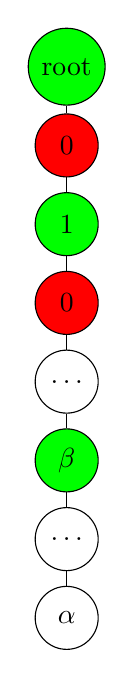
\begin{tikzpicture}[every node/.style={circle,draw,minimum size = 8 mm}]
  \node [fill = green](root) at (1,0) {root};
    \node [fill=red](zero) at (1,-1) {$0$};
    \node [fill=green](one) at (1, -2) {$1$};
    \node [fill=red](zero2) at (1,-3) {$0$};
    \node(dots) at (1,-4) {$\ldots$};
    \node[fill=green](beta) at (1,-5) {$\beta$};
    \node (dots2) at (1,-6) {$\ldots$};
    \node (alpha) at (1, -7) {$\alpha$};
    \draw (root) -- (zero);
    \draw (zero) -- (one);
    \draw (one) -- (zero2);
    \draw (zero2) -- (dots);
    \draw (dots) -- (beta);
    \draw (beta) -- (dots2);
    \draw (dots2) -- (alpha);
\end{tikzpicture}
    \caption{Legitimate alternating path}
    \label{fig:legitimate_alternating_path}
\end{subfigure}
\hfill
\begin{subfigure}[b]{0.3\textwidth}
\centering
    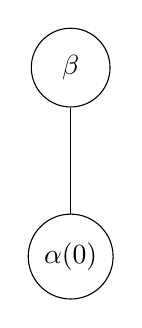
\begin{tikzpicture}[yscale=1.2,every node/.style={circle,draw,minimum size = 10 mm}]
  \node (b) at (1,0) {$\beta$};
    \node (a) at (1,-2) {$\alpha(0)$};
    \draw (b) -- (a);
\end{tikzpicture}
\quad
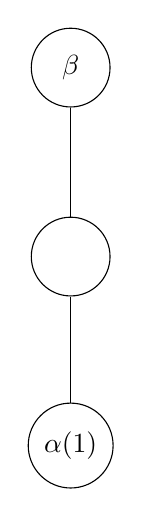
\begin{tikzpicture}[yscale=1.2,every node/.style={circle,draw,minimum size = 10 mm}]
  \node (b) at (1,0) {$\beta$};
  \node (c) at (1, -2) {};
    \node (a) at (1,-4) {$\alpha(1)$};
    \draw (c) -- (a);
    \draw (b) -- (c);
\end{tikzpicture}
    \caption{Parent or grandparent of $\alpha$ is $\beta$}
    \label{fig:parent_alpha}
\end{subfigure}
\hfill
\begin{subfigure}[b]{0.3\textwidth}
    \centering
    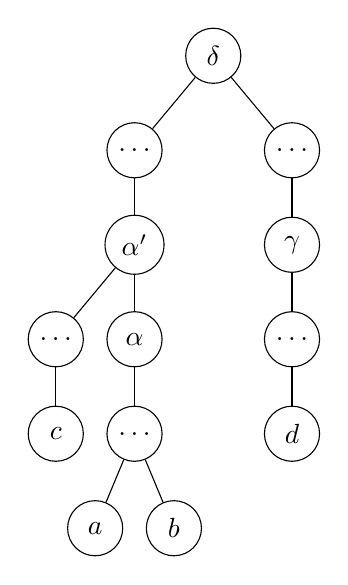
\begin{tikzpicture}[yscale=1.2,every node/.style={circle,draw,minimum size = 7 mm}]
  \node (b) at (1,0) {$\delta$};
    \node (a) at (0,-3) {$\alpha$};
    \node (pa) at (0, -2) {$\alpha'$};
    \node (e) at (0, -1) {$\ldots$};
    \node (e2) at (2, -1) {$\ldots$};
    \node (e3) at (-1, -3) {$\ldots$};
    \node (g) at (2, -2) {$\gamma$};
    \node (c) at (-1, -4) {$c$};
    \node (e4) at (0,-4) {$\ldots$};
    \node (reala) at (-0.5,-5) {$a$};
    \node (realb) at (0.5,-5) {$b$};
    \node (e5) at (2, -3) {$\ldots$};
    \node (d) at (2, -4) {$d$};
    \draw (g) -- (e5);
    \draw (e5) -- (d);
    \draw (e4) -- (realb);
    \draw (e4) -- (reala);
    \draw (a) -- (e4);
    \draw (e) -- (pa);
    \draw (b) -- (e);
    \draw (b) -- (e2);
    \draw (e2) -- (g);
    \draw (pa) -- (e3);
    \draw (e3) -- (c);
    \draw (a) -- (pa);
\end{tikzpicture}
    \caption{Proving existance of $P_4$ in condition $1$ of the theorem \ref{theorem_adding_equivalent}}
    \label{fig:theorem_1}
\end{subfigure}
\caption{Examples of cograph structure}
\end{figure}



\begin{theorem}[Theorem 1 \cite{corneil_perl_stewart_85}]
    \label{theorem_adding_equivalent}
     The given graph $G$ is a cograph if and only if none of the following conditions are true:
    
\begin{enumerate}
    \item there exists a $(0)$-node in $M \setminus \{\alpha\}$,
    \item there exists $v \in$ $ M \setminus \{\alpha\}$, such that $v$ is a $(1)$-node and is not properly marked,
    \item there exists $y \in M \setminus \{\alpha\}$, such that $y \neq R$ and the grandparent of $y \notin M \setminus \{\alpha\}$,
    \item The vertices of $ M \setminus \{\alpha\}$ do not lie on one path to $R$,
    \item $\alpha$ is a $(0)$-node whose parent is not $\beta$,
    \item $\alpha$ is a $(1)$-node which has a grandparent which is not $\beta$.
\end{enumerate}
\end{theorem}
It is easy to prove that this theorem is equivalent to the \Cref{theorem_adding}.

\subsection{Theorem \ref{theorem_adding_equivalent}}
Now let us prove that if condition $1$ of the Theorem \ref{theorem_adding_equivalent} is true, then $G$ is not a cograph. The other cases are similar.

From now on let $des (x)$ denote the leaves of the subtree of $x$, $\gamma$ be some $(0)$-node in $M \setminus \{\alpha\}$ and $\delta$ be the LCA of $\alpha$ and $\gamma$. 

We have to consider four cases, depending of what label do $\alpha$ and $\delta$ have. Here we consider their labels are both $0$ (see \Cref{fig:theorem_1}). The other cases follow similarly.

Let $\alpha'$ be the parent of $\alpha$. As it was said above, if all leaves in the subtree are the neighbours of $x$, then this node is ``marked-and-unmarked'', but we look at the nodes in $M$. Such nodes have at least one neighbour of $x$ and one not neighbour of $x$ in their subtrees. So, $a \in des(\alpha)$ is the neighbour of $x$,$b \in des(\alpha)$ is not a neighbour of $x$, $c \in des (\alpha') \setminus des(\alpha)$, $d \in des (\gamma)$ (except one case under) is the neighbour of $x$. If c is the neighbour of $x$, the $P_4$ is $b-c-x-d$, else $b-c-a-x$. But if $\delta = \gamma$,  $d \in des(y) \setminus des(\theta)$, where $\theta$ is the child of $\gamma$ on the $\alpha - \gamma$ path. 



\subsection{\texttt{FIND-LOWEST}}
Function \texttt{FIND-LOWEST} finds $\alpha$, the lowest marked node of cotree. 

\subsection{\texttt{ADD-VERTEX}}
Let us prove of one of many cases of the function \texttt{ADD-VERTEX} -- when $u$ is a $(0)$-node and the size of $A[0]$ does not equal to $1$. The other cases are similar. We use the notation from function \texttt{ADD-VERTEX} implementation. 
\begin{theorem}
    For each pair of leaves $(a,b)$ in the modified cotree $T'$, where $x \notin \{a, b\}$, the labels of LCA$_T(a,b)$ and LCA$_{T'}(a,b)$ are the same.
\end{theorem}
\begin{proof}
We call a vertex \emph{beautiful} if it is from the subtree of some vertex from $A[0]$ and \emph{ugly} if it is from the subtree of some child of $u$, such that $u$ is not in $A[0]$.

There are two states of every vertex -- is in the subtree of $u$, which in turn divided into beautiful and ugly, and is not in the subtree of $u$.
        \begin{itemize}
            \item if $a$ and $b$ are not from the subtree of $u$, then their LCA stays the same,
            \item If exactly one node (only $a$ or only $b$) is from the subtree of $u$ and the other is not from subtree of $u$, then their LCA is still the same,
            \item if $a$ and $b$ are both beautiful or both ugly, then if their LCA is not $u$, then it remains the same. If their LCA is $u$, then if $a$ and $b$ are beautiful, it becomes $y$, that has the same label as $u$; and if $a$ and $b$ are ugly, then their LCA is still $u$.
            \item if exactly one between $a$ and $b$ is beautiful and the other is ugly, then their LCA is still $u$.
        
        \end{itemize}
From the description of the algorithm, all vertices from $A[0]$, i.e. beautiful ones are now the children of $y$. Now we consider a beautiful node $l$ and an ugly node $r$ (see \Cref{fig:ADD-VERTEX}). $L(l)$ are all neighbours of $x$, because $l$ is ``marked-and-unmarked''. There are no neighbours of $x$ in $L(r)$, because $r$ is ``unmarked''.
\end{proof}
Now it's time to consider the case when $a=x$ or $b=x$. 
\begin{theorem}
    For every $b \neq x$ from $L(u)$, the label of the LCA of $x$ (the vertex that we are inserting to the cograph) and $b$, is correct.
\end{theorem}
\begin{proof}
Let us split the proof into the several cases:
        \begin{itemize}
            \item If $b$ is from $L(l)$ then their LCA is a new $(1)$-node and it is correct, because in $L(l)$ are only neigbours of $x$,
            \item If $b$ is from $L(r)$ then their LCA is $u$ and it is correct, because $u$ is $(0)$-node and in $L(r)$ there are no neighbours of $x$,
        \item If $b$ is not from $L(u)$, then we know that the path between $u$ and $R$ is a legitimate alternating path. 
        \begin{itemize}
            \item If the LCA of $x$ and $b$ is a $(0)$-node, and we know it is not marked, i.e. among its children there are not ``marked-and-unmarked'' vertices. Due to the existence of a legitimate alternating path we know than in the subtree of LCA,  excluding the subtree of its properly marked $(1)$-node, there are no ``marked'' vertices.  Therefore, every such child of LCA is ``unmarked'', and this logic can be recursively applied conclude that $L(LCA)$ has no neighbours of $x$, making it the correct LCA,
            \item If the LCA is a $(1)$-node, and we know it is properly marked, it has exactly one not ``marked-and-unmarked'' child, and this child is an ``unmarked'' $(0)$-node and the other children are ``marked-and-unmarked''. For every such child $c$ we know that $L(c)$ consists only of neighbours of $x$, making it the correct LCA too.
        \end{itemize}
        \end{itemize}
\end{proof}
        
\begin{figure}
    \centering
    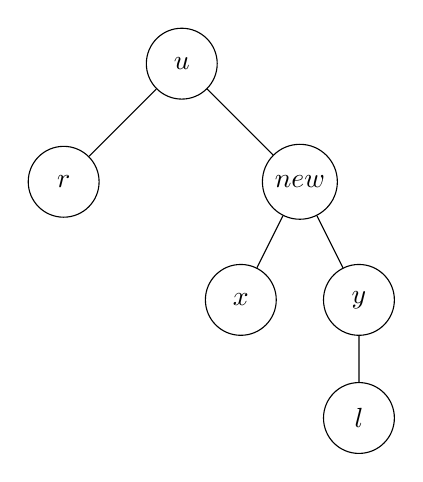
\begin{tikzpicture}[xscale=1.5,every node/.style={circle,draw,minimum size=9mm}]
  \node (u) at (1,0) {$u$};
  \node (l) at (2.5, -4.5) {$l$};
  \node (r) at (0, -1.5) {$r$};
  \node (new) at (2,-1.5) {$new$};
  \node (x) at (1.5,-3) {$x$};
  \node (y) at (2.5,-3) {$y$};

    \draw (y) -- (l);
    \draw (u) -- (r);
  \draw (u) -- (new);
  \draw (new) -- (x);
  \draw (new) -- (y);
\end{tikzpicture}
    \caption{\texttt{ADD-VERTEX} special case proof}
    \label{fig:ADD-VERTEX}
\end{figure}        

\section{Complexity}
\begin{theorem}
    Each iteration takes $O(\deg(x))$ time.
\end{theorem}
\begin{proof}
\texttt{MARK}: each node except root has a minimum of two children. If we imagine that all vertices, which are not neighbours of $x$ don't exist, then the tree has $\deg(x)$ leaves and the previous layer has at most $\frac{\deg(x)}{2}$ vertices, the one before that has at most $\frac{\deg(x)}{4}$ and so on. To calculate the total complexity we need to sum $\deg(x) + \frac{\deg(x)}{2} + \frac{\deg(x)}{4} + \dots$, which forms a geometric progression. The sum is at most $2 \cdot \deg(x)$, so it is $O(\deg(x))$. Therefore, the size of $M$ is also $O(\deg(x))$. For each node, processing time is $O(1)$, and the total time complexity of this function is $O(\deg(x))$.

\texttt{FIND-LOWEST}: each node from $M$ is processed in $O(1)$ time, the total complexity of this function is also $O(\deg(x))$.

\texttt{ADD-VERTEX}: all cases of inserting require $O(1)$ time, but the operation of removing elements of $A$ from $u$ to $y$ is $O(\deg(x))$, because $|A| \leq |M|$. 

\end{proof}
Therefore, the total time complexity of the algorithm is $O( \sum\limits_{v \in V}^{} \deg(v)) = O(n+m)$.
